\label{key}\documentclass[letterpaper, 12pt,oneside]{article}
\usepackage{amsmath}
\usepackage{graphicx}
\usepackage{xcolor}
\graphicspath{{Imagenes/}}
\usepackage[utf8]{inputenc}
\usepackage{listings}
\usepackage[hidelinks]{hyperref}

\title{\Huge Taller de Herramientas Computacionales}
\author{Josué Artemio Hernández Rodríguez}
\date{24/Enero/2019}

\begin{document}
	\maketitle
	\begin{center}
		
\includegraphics[scale=0.7]{3.jpg}
	\end{center}

	\newpage
	
	\title{\huge \textit{Bitácora problema 5 }}\\

	Este problema te calcula la suma de los n primeros naturales. No se si el profesor menciono algo al respecto al prohibir usar este método, pero lo que hice fue colocar la formula que te calcula directamente, aunque puede hacerse de otra forma, con una función recursiva por ejemplo, o con un for. La solución solo te pide que número y te calcula la suma de esos n naturales. 
	
	 

	\begin{figure}[h]
		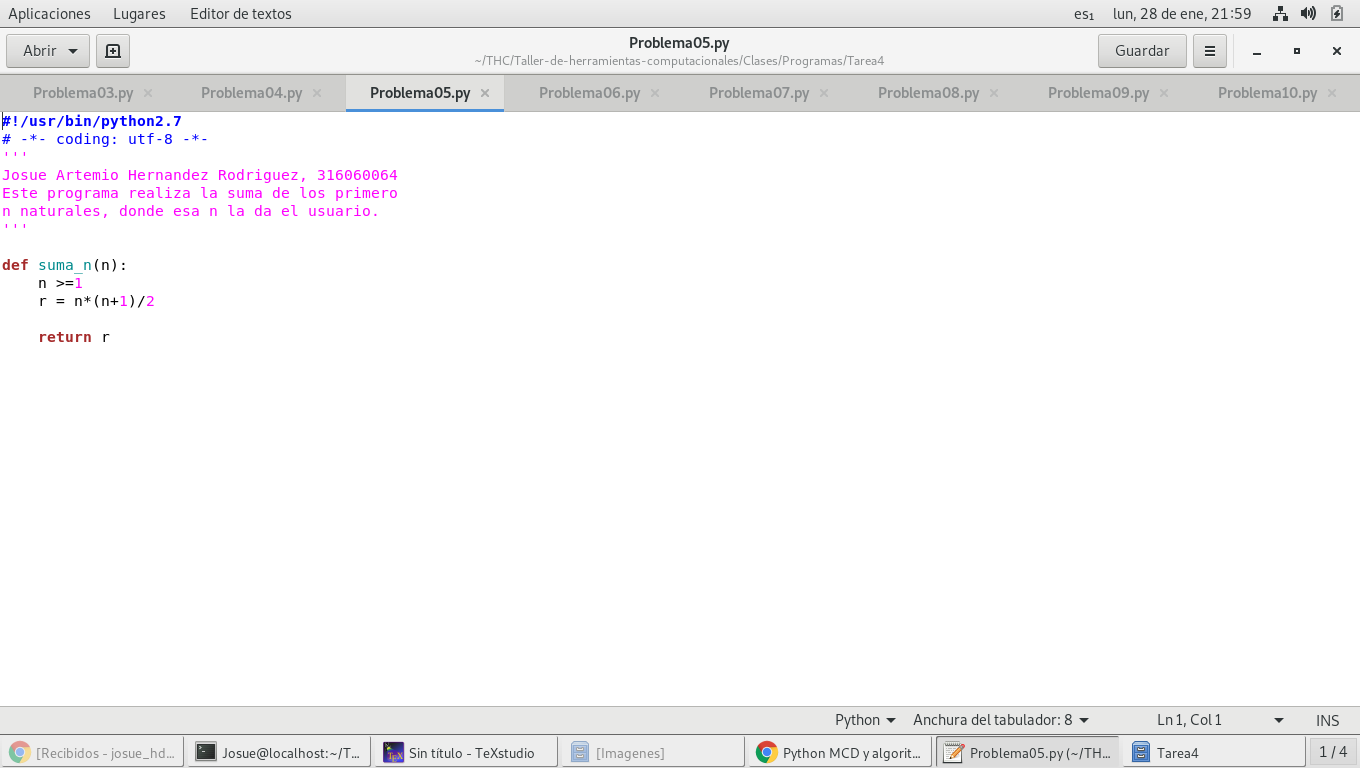
\includegraphics[scale=0.3]{pro05.png}
	\end{figure}
	
	
	
	
	
	
	
	
	
	
	
\end{document}
